% pdflatex tabpfn_distilasi_angular.tex
% pdftoppm -png -r 300 -singlefile tabpfn_distilasi_angular.pdf tabpfn_distilasi_angular
\documentclass[border=7pt]{standalone}
\usepackage{mathptmx}
\usepackage{tikz}
\usetikzlibrary{arrows.meta,shadows}

\definecolor{ink}{HTML}{3A3936}
\definecolor{muted}{HTML}{656461}
\definecolor{dataF}{HTML}{F0EFEC}
\definecolor{modelE}{HTML}{2A78D6}\definecolor{modelF}{HTML}{DCE9F9}
\definecolor{augE}{HTML}{EB6834}\definecolor{augF}{HTML}{FDE3D6}
\definecolor{opE}{HTML}{6250D6}\definecolor{opF}{HTML}{EBE9FB}
\definecolor{lossE}{HTML}{1BAF7A}\definecolor{lossF}{HTML}{D9F3E9}

\tikzset{
  every node/.style={font=\small,text=ink,align=center},
  base/.style={rectangle,rounded corners=3pt,minimum height=12mm,inner sep=3pt,line width=0.8pt},
  data/.style={base,fill=dataF,draw=muted,text width=23mm},
  model/.style={base,fill=modelF,draw=modelE,text width=25mm},
  aug/.style={base,fill=augF,draw=augE,line width=1.2pt,text width=24mm},
  target/.style={base,fill=opF,draw=opE,text width=42mm},
  loss/.style={base,fill=lossF,draw=lossE,text width=30mm},
  tensor/.style={rectangle,fill=white,draw=modelE,line width=.8pt,minimum width=7mm,minimum height=9mm,
    double copy shadow={shadow xshift=1.5pt,shadow yshift=1.5pt,draw=modelE,fill=white}},
  flow/.style={-{Stealth[length=2.3mm]},line width=.8pt,draw=ink,rounded corners=4pt},
  fixed/.style={flow,densely dashed,draw=opE},
  note/.style={font=\footnotesize\itshape,text=muted},
}
\newcommand{\sub}{\footnotesize\color{muted}}

\begin{document}
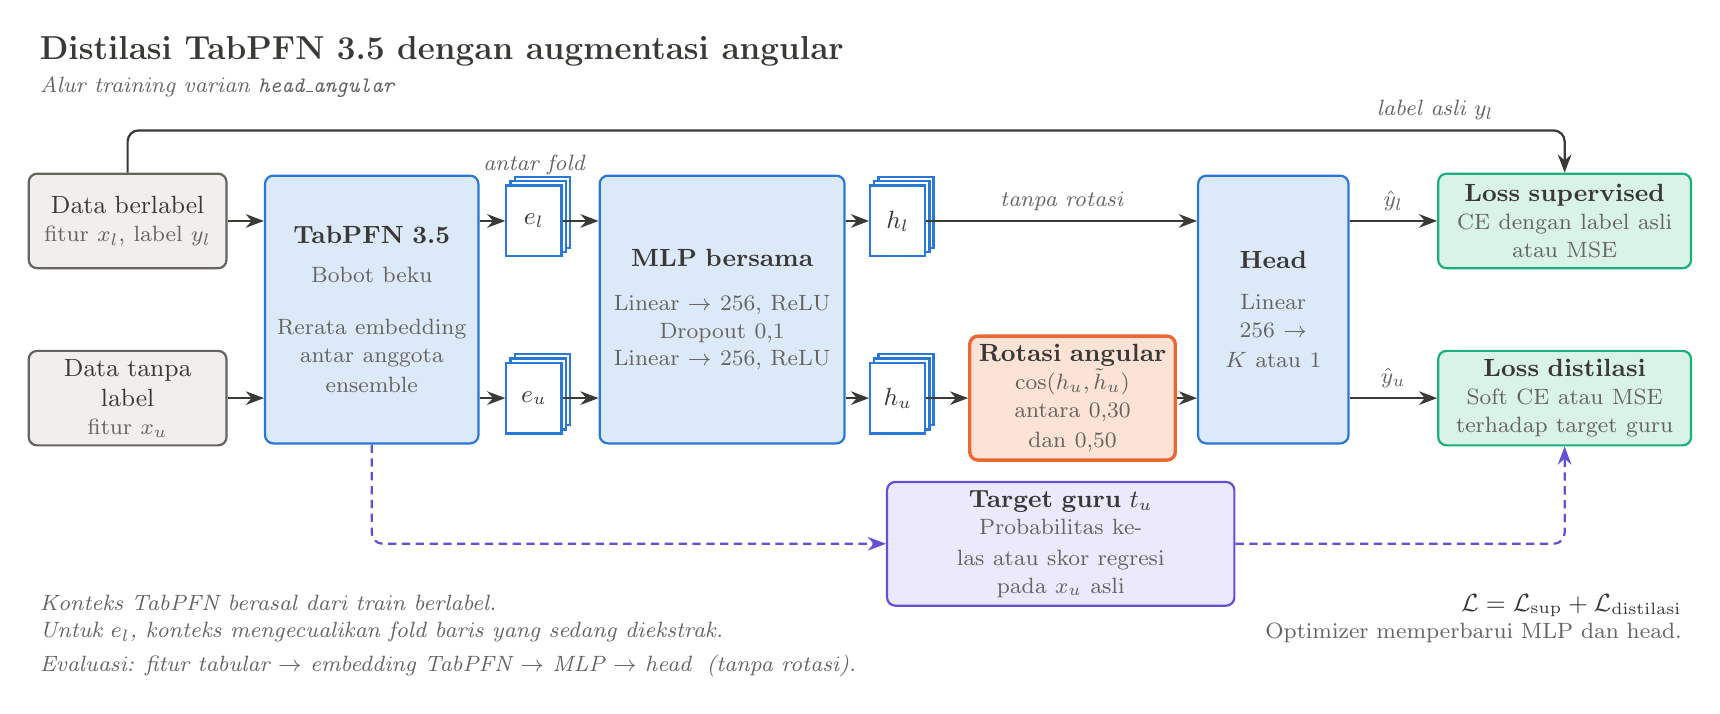
\begin{tikzpicture}
\def\yU{-2.25}
\def\yTeacher{-4.1}

\node[anchor=west,font=\large\bfseries] at (-1.24,2.15) {Distilasi TabPFN 3.5 dengan augmentasi angular};
\node[note,anchor=west] at (-1.24,1.70) {Alur training varian \texttt{head\_angular}};

\node[data] (xl) at (0,0) {Data berlabel\\[-1pt]{\sub fitur $x_l$, label $y_l$}};
\node[data] (xu) at (0,\yU) {Data tanpa label\\[-1pt]{\sub fitur $x_u$}};
\node[model,minimum height=34mm] (pfn) at (3.1,-1.125)
  {\textbf{TabPFN 3.5}\\[3pt]{\sub Bobot beku}\\[8pt]{\sub Rerata embedding}\\[-1pt]{\sub antar anggota ensemble}};
\node[tensor] (el) at (5.16,0) {$e_l$};
\node[tensor] (eu) at (5.16,\yU) {$e_u$};
\node[note,above] at (el.north) {antar fold};

\node[model,text width=29mm,minimum height=34mm] (mlp) at (7.55,-1.125)
  {\textbf{MLP bersama}\\[5pt]{\sub Linear $\to$ 256, ReLU}\\[-1pt]{\sub Dropout 0,1}\\[-1pt]{\sub Linear $\to$ 256, ReLU}};
\node[tensor] (hl) at (9.78,0) {$h_l$};
\node[tensor] (hu) at (9.78,\yU) {$h_u$};
\node[aug] (angular) at (12.00,\yU)
  {\textbf{Rotasi angular}\\[-1pt]{\sub $\cos(h_u,\tilde h_u)$}\\[-1pt]{\sub antara 0,30 dan 0,50}};
\node[model,text width=17mm,minimum height=34mm] (head) at (14.55,-1.125)
  {\textbf{Head}\\[4pt]{\sub Linear}\\[-1pt]{\sub 256 $\to$ $K$ atau 1}};

\node[loss] (sup) at (18.25,0) {\textbf{Loss supervised}\\[-1pt]{\sub CE dengan label asli}\\[-1pt]{\sub atau MSE}};
\node[loss] (dist) at (18.25,\yU) {\textbf{Loss distilasi}\\[-1pt]{\sub Soft CE atau MSE}\\[-1pt]{\sub terhadap target guru}};
\node[target] (teacher) at (11.85,\yTeacher)
  {\textbf{Target guru $t_u$}\\[-1pt]{\sub Probabilitas kelas atau skor regresi}\\[-1pt]{\sub pada $x_u$ asli}};

\draw[flow] (xl.east) -- (xl -| pfn.west);
\draw[flow] (xu.east) -- (xu -| pfn.west);
\draw[flow] (pfn.east |- el) -- (el.west);
\draw[flow] (pfn.east |- eu) -- (eu.west);
\draw[flow] (el.east) -- (el -| mlp.west);
\draw[flow] (eu.east) -- (eu -| mlp.west);
\draw[flow] (mlp.east |- hl) -- (hl.west);
\draw[flow] (mlp.east |- hu) -- (hu.west);
\draw[flow] (hl.east) -- node[note,above] {tanpa rotasi} (hl -| head.west);
\draw[flow] (hu.east) -- (angular.west);
\draw[flow] (angular.east) -- (angular -| head.west);
\draw[flow] (head.east |- sup) -- node[note,above] {$\hat y_l$} (sup.west);
\draw[flow] (head.east |- dist) -- node[note,above] {$\hat y_u$} (dist.west);
\draw[flow] (xl.north) -- (0,1.15) -- node[note,above,pos=.91] {label asli $y_l$} (18.25,1.15) -- (sup.north);
\draw[fixed] (pfn.south) |- (teacher.west);
\draw[fixed] (teacher.east) -| (dist.south);

\node[note,anchor=west,align=left] at (-1.24,-5.05)
  {Konteks TabPFN berasal dari train berlabel.\\Untuk $e_l$, konteks mengecualikan fold baris yang sedang diekstrak.};
\node[anchor=east,align=right] at (19.86,-5.05)
  {$\mathcal L=\mathcal L_{\mathrm{sup}}+\mathcal L_{\mathrm{distilasi}}$\\[-1pt]
   {\sub Optimizer memperbarui MLP dan head.}};
\node[note,anchor=west] at (-1.24,-5.65)
  {Evaluasi: fitur tabular $\to$ embedding TabPFN $\to$ MLP $\to$ head \;(tanpa rotasi).};
\end{tikzpicture}
\end{document}
